% $Id: preview.tex,v 1.19 1998/06/22 08:07:00 ohl Exp $
%%%%%%%%%%%%%%%%%%%%%%%%%%%%%%%%%%%%%%%%%%%%%%%%%%%%%%%%%%%%%%%%%%%%%%%%


\NeedsTeXFormat{LaTeX2e}
\documentclass[11pt]{article}
\usepackage{amsmath,amssymb,amsthm}
\usepackage[margin=1.0in]{geometry}
\usepackage{amscd}
\usepackage{epsfig}
\allowdisplaybreaks
\setlength{\unitlength}{1mm}
%%%%%%%%%%%%%%%%%%%%%%%%%%%%%%%%%%%%%%%%%%%%%%%%%%%%%%%%%%%%%%%%%%%%%%%%
\makeindex
\begin{document}
\title{\bf {PURE DATA FOUNDATIONS OF MATHEMATICS}}
\author{%
  Saul Youssef%
  \hfil \\
  Department of Physics \\
  Boston University \\
  youssef@bu.edu\\
}
\maketitle
\begin{abstract}
This is an abstract.
\end{abstract}
%%%%%%%%%%%%%%%%%%%%%%%%%%%%%%%%%%%%%%%%%%%%%%%%%%%%%%%%%%%%%%%%%%%%%%%%

%%%%%%%%%%%%%%%%%%%%%%%%%%%%%%%%%%%%%%%%%%%%%%%%%%%%%%%%%%%%%%%%%%%%%%%%
\section{Introduction}

\section{Foundation}

     Any system of reasoning must necessarily have at least one foundational concept which is understood before a first definition.  In our case, the foundational concept is the {\it finite sequence}.  We assume that finite sequences and obvious operations on finite sequences are understood.  On the other hand, logic, logical values and predicates (foundational in ZFC) and types (foundational in type theories) will be defined in terms of finite sequences.
Taking finite sequences as understood, define `data' and `coda' by the following.
\begin{itemize}
\item {\it Data} is a finite sequence of {\it codas}, and a {\it coda} is a pair of {\it data}. 
\end{itemize}
Notationally speaking, if $A$ and $B$ are data, $A\ B$ denotes the concatenation of $A$ and $B$ as finite sequences and $A:B$ denotes the data
consisting of the single coda formed by pairing $A$ and $B$.  By the definition, for example, the empty sequence of codas $()$ is data, and, therefore,
so is the pairing of two empty sequences `$(:)$' and so is this sequence of three codas $(:) (:) ((:):(:))$.  We shall refer to this as ``pure data'' 
since it is data ``made from finite sequences of nothing."    
We shall see that both data in the ordinary sense (bits, bytes, language expressions) and mathematical concepts such as variables, functions, definitions, logical values, categories, morphisms, types and theorems naturally appear as varieties of pure data with simple definitions expressed in the small algebra
of data with the concatenation and the colon operations.   Notationally speaking, the colon operation binds from the right first and binds 
less strongly than concatenation, so that
 $A:B:C$ means $(A:(B:C))$ and $A:B\ C$ means $(A:(B\ C))$.

     In coda, the answers to mathematical questions come from an equivalence relation $=$, which is defined by a partial function from codas to data
called a {\it context}.  Given a context $\delta$, equality is defined by
\begin{equation} \label{eqn}
	A\ B = \delta(A)\ B = A\ \delta(B)
\end{equation}
\begin{equation} \label{eqn}
	A:B = \delta(A):B = A:\delta(B)
\end{equation}
for data $A$ and $B$ where the partial function $\delta$ has been extended to a function from data to data with identities.
Conceptually, relations are assumed until $\delta$ is an identity on data.  With a given context, data $A$ is {\it empty} if $A=()$ and {\it invariant}
if $\delta(A)=A$.

     In coda, new definitions are added to a context as partial functions from codas to data.  We use a convention to guarantee that each such partial
function has it's own disjoint domain.  Let the {\it domain} of a coda $A:B$ be the data consisting of the first coda in the sequence $A$ and the empty
sequence if $A$ is empty.  A partial function mapping the all of the codas with a particular invariant domain to data is called a {\it definition}.  Definitions
can be added to a valid context if they do not clash with previous definitions.

\newtheorem*{remark}{THE AXIOM OF DEFINITION}
\begin{remark}  The empty context is valid.  If $\delta$ is a valid context and $d$ is a definition, and if no coda is in
the domain of both $\delta$ and $d$, then the union of $\delta$ and $d$ is a valid context.
\end{remark}
\noindent As an axiomatic system, coda is complete at this point.  This is quite a contrast from, for instance, ZFC which has ten axioms 
even assuming predicate logic.  The reason for the simplification will become clear in the sections which follow.  In section 4, we show 
that coda already has an internal logic implicit in the structure as defined.  We adopt this logic for reasoning within coda, so we do not 
need axioms related to propositional or predicate logic.  In section 5, we show that coda also contains an internal language which can 
also be defined just as with any other definition.  The language has the unusual property that all byte sequences are valid syntax, 
so language and language syntax axioms are also not needed.  Axioms specifying valid ``rules of deduction'' are also not needed 
because deduction, proof, and computation in coda are all determined by the above data equality.  Each of these is a merely a data sequence $A_0=A_1=A_2=\dots=A_n$, 
deducing $A_n$ from $A_0$, computing $A_n$ starting with $A_0$ or proving that $A_0=A_n$, depending on one's point of view.  
Unlike type systems with a Curry-Howard correspondence, proof and computation are the same thing in coda. 

In the sections that follow, 
``data" and ``pure data'' are interchangeable terms and ``sequence'' will always mean a finite sequence unless otherwise indicated.  Since coda 
only has one axiom, we may refer to the Axiom of Definition as just ``the axiom.'' 

\section{Definitions} 

      As specified in the Axiom of Definition, a definition is specified by a) choosing invariant data to be the domain of the definition and b) specifying a function from 
 codas with that domain to pure data.  For example, we can define that any coda with domain $()$ maps to itself.  This establishes that $(:B)$ as an atom for any 
 data $B$, and if $B$ is invariant, then so is the coda, so $(:)$, for instance, is invariant and can be the domain of more definitions. Continuing in this fashion, we define 
 codas with domain $(:)$ to be ``bits'', so $(:):$ is the 0-bit, $(:):(:)$ is the 1-bit.  Codas with the 0-bit as domain are conventionally bit sequences and codas with 
 domain 1-bit are conventionally byte sequences.  This makes byte strings available as invariant names for other definitions.  For instance, by 
 {\bf (pass A:B)$\rightarrow$ B} we mean a definition so that any coda with domain ``pass'' maps (pass A:B) to B.  If ``pass'' has not already been used, this 
 definition may be added to context.  It can be helpful to think of {\bf pass} as a ``command'' with ``input'' B and ``argument'' A.  
Typical examples are shown in table X.  
\begin{table}
\begin{tabular}{ | l | l | l | }
Domain & Description & Action \\
\hline
pass & Pass input unchanged & (pass A:B)$\rightarrow$ B \\
\hline
null & Empty data for any input & (null A:B)$\rightarrow$ () \\
\hline
rev & Reverse the order of data & (rev : B)$\rightarrow$ (), if B is empty \\
 &  & (rev : b)$\rightarrow$ b, if b is an atom \\
 & & (rev : B C)$\rightarrow$ (rev:B) (rev:A) \\ 
 \hline
 if & Conditional B & (if A:B) $\rightarrow$ B, if B is empty \\
 & & (if A:B) $\rightarrow$ (), if B is atomic. \\
 \hline 
 ap & Apply argument A to each input & (ap A : B)$\rightarrow$ (), if B is empty \\
  & & (ap A : b)$\rightarrow$ A:b, if b is an atom \\
  & & (ap A : B C)$\rightarrow$ (ap A:B) (ap A:C) \\  
\hline
nat & The natural numbers & (nat : $n$)$\rightarrow$ $n$ (nat\ :\ $n+1$) \\
\hline
def & Make a new definition & (def A:B)$\rightarrow$ add definition (A $A'$:$B'$)$\rightarrow$ B. \\
\hline 
\end{tabular}
\caption{\label{ }{\it Typical definitions in coda.  Each definition is a partial function from codas to data defined on  
codas with a specified domain.  When multiple actions are listed, the total action is defined by the first action 
where the left hand side pattern applies.}}
\end{table}
In addition to the approximately 50, very simple, pre-defined built in definitions, coda includes a definition (def A : B) which lets one 
add new definitions to a context provided that A is invariant and not already used in the context, according to the Axiom of Definition.
A particularly important and typical family of definitions are the {\it applications} such as {\bf ap} in Table 2.  These 
are simple combinatorial operations on sequences.  Taking finite sequences as understood, we presume that descriptions 
such as those in Table 2 are sufficient for a clear understanding of the meaning of these sorts of definitions.  Of course, further description and built in examples are available with the software, and the source code implementation of these is also always 
short and readable.  
\begin{table}
\begin{tabular}{| l  l  l | }
Schematic Coda & $\rightarrow$ & Schematic Result \\
\hline
ap A:$b_1$ $b_2$ $b_3$ & $\rightarrow$ & (A:$b_1$) (A:$b_2$) (A:$b_3$) \\
app $a_1$ $a_2$ $a_3$:B &  $\rightarrow$ & ($a_1$:B) ($a_2$:B) ($a_3$:B) \\
ap2 $a$ $a_1$ $a_2$ $a_3$:B & $\rightarrow$ & ($a$ $a_1$:$b_1$) ($a$ $a_2$:$b_2$) ($a$ $a_3$:$b_3$) \\
aps A:$b_1$ $b_2$ $b_3$ $b_4$ & $\rightarrow$ & (A $b_1$:(A $b_2$ : (A $b_3$:$b_4$))) \\
apif A:$b_1$ $b_2$\dots & $\rightarrow$ & $b_1$ (\dots if (A:$b_1$) is empty) $b_2$ (\dots if (A:$b_2$) is empty) \dots \\
\hline
\end{tabular} 
\caption{\label{ }{\it Typical combinatoric definitions combine data A and B as sequences.}}   
\end{table}

\section{Logic}

The previous sections can be simply summarized.  We have recursively defined ``pure data'' to be finite sequences of pairs of pure data called codas.  Given such 
data,  any partial function from coda to data qualifies as a ``definition.''  Under the conditions of the Axiom of Definition, definitions can be added to 
a ``context'' which defines an equality on data and meaning within the system.  
These simple definitions and, for instance, the combinatorial examples in figure 1 are meant to be sufficiently understood based on the foundational concept 
of the {\bf finite sequence} without the need for logical axioms or logical values.   We presume, for instance, that reversing the order of a finite 
sequence is understood without making a choice between, say, classical and intuitionistic logic.  

    In the framework of coda, all mathematical objects (values, functions, variables, morphisms, theorems,\dots) are meant to be merely pure data.  This means 
that ``propositions" will appear in the form: 
\begin{itemize}
\item[] Is data $A$ equal to data $B$?
\end{itemize}
Since equality itself is available as a definition, then this question is also the specific data $A=B$ or $(=A:B)$.  But if a question like ``Is data $A$ equal to data $B$?" is data, 
it is natural to expect that the answer to the question should be encoded in the specific data $(=A:B)$.  This suggests that ``logic'' in coda should appear as 
a natural coarse classification of data in general.  The classification should match our intuition and ordinary reasoning and should be stable under 
adding new definitions to a given context.  A suitable classification is indeed available.  

     Given a particular context, data $A$ is said to be {\it atomic} if one or more of the codas in it's sequence is invariant.  Note that since being empty and being atomic 
are disjoint categories which are preserved when adding new definitions to a context, this classification is an interesting candidate: 
\begin{itemize}
\item data is {\it true} if it is empty, {\it false} if it is atomic and {\it undecided} otherwise. 
\end{itemize}
although true data is ``always true" and false data is ``always false," [always], undecided data may become true or false with added 
definitions.  In this sense, undecided data are like ``variables'' which may receive a true or false value depending on future choices.  
This is not quite the correct picture, however, because some undecided data actually remain undecided independent of any future added definitions.  
Such {\it undecidable} data occurs, for example, with the Godel phenomenon as we shall see in section Y.  
The fact that coda logic is "almost" two-valued logic is from the duality between {\it true} data $()$  and {\it false} data $(:)$ visible in any display of pure data.  
Although proposing to change something as fundamental as logic can be disorienting, one soon realizes that the situation is still quite familiar and that the 
seemingly odd ``undecided'' category works perfectly.  
Examples illustrate the flavor of these definitions assuming a context where "a", "b", "c" and "foo" and "bar" are not the domains of a definition in context: 
\begin{center}
\begin{tabular}{ | c | c | }
\hline
 {\it True} & (), ({\bf pass}:), {\bf null} : a b c, ({\bf and}:), ({\bf or} a:), ({\bf xor} : a)  \\ 
 \hline
 {\it False} & a b c, {\bf first} 3 : a b (foo:bar), ({\bf and} a:b), ({\bf or} a:b)  \\  
 \hline
 {\it Undecided} & foo:bar, {\bf pass}:foo:bar, {\bf last}:a b (foo:bar)  \\   
 \hline
\end{tabular}
\end{center}
In the above , ``and'', ``or'', and ``xor'' are familiar binary operations from classical logic in the cases where their arguments are true or false in the coda sense. 
For instance, if data $A$ and $B$ are both either true or false then $({\rm xor}\ A:B)$ is $()$ for {\it true} and $(:)$ for {\it false} according to the standard truth
 table for the {\bf xor} operation.  On the other hand, if either $A$ or $B$ are 
undecided, the data $({\rm xor}\ A:B)$ has no definitions that apply.  In effect, $({\rm xor}\ A:B)$ ``waits" until both $A$ and $B$ are defined enough to have logical values.   
This is an example where $({\rm xor}\ A:B)$ acts as a logical expression with ``variables'' $A$ and $B$. 

Undefined data may occur even when data does not explicitly contain an undefined coda such as (foo:bar) above. For example 
the natural numbers in coda is the data (nat:0) because a definition $({\rm nat}:n)\rightarrow n\ ({\rm nat}:n+1)$ means that (nat:0) = 0 1 2 3 4 5 (nat:6), etc.  
The sum of the first 1000 natural numbers is perfectly well defined and is computed by ``sum n : first 1000 : nat : 0''.  What happens, however, 
if we decided to sum all natural numbers via ``sum n : nat : 0"?  The answer is that this data remains undecided no matter how much the 
expression is evaluated.  Here, the undecided logical category is, quite nicely and naturally, the logical value of data that is not defined.  

Classical logic can be thought of as establishing at least two things: 1) defining how to reason correctly and 2) assigning logical meaning to ``propositions.''  
Within coda, 1) reasoning is correct if and only if it is application of a definition in context and 2) logical meaning is defined by data being either empty, atomic or neither.  
Rather than propositions being foundational undefined entities, propositions in coda are just data and their logical values are also just data.  
There is an understandable and perhaps even unpleasant disorientation caused by attempting to re-defining something 
as fundamental as classical logic.  We have found that this disorientation is only temporary once one realizes that the familiar binary logical operations remain,
 and the seemingly odd class of ``undecided'' data fits in perfectly as ``logic valued variables" and as ``the answers to questions that have no answers."  Confidence may 
 be gained in section X where we examine Godel phenomena and directly compute some paradoxes. 

\section{Language}

Both predicate logic with ZFC or with dependent type theory are formal languages.  They have alphabets with special symbols 
and axiomatic syntax rules which 
distinguish meaningful sentences from nonsense sentences such as ``$xyxy\forall\exists\exists x x\forall$''.  The situation with coda is 
much simpler because we can define the language itself as an ordinary definition, added to a context via the Axiom of Definition just 
like all other definitions.  The basic idea behind the language definition is to give textual control over the concatenation and colon operations.
Thus, if $x$ and $y$ are language expressions, partial functions 
\begin{equation} \label{eqn} 
( \{x\ \ y\} \ A : B ) \rightarrow (\{x\}\ A : B)\ (\{y\}\ A : B)
\end{equation} 
\begin{equation} \label{eqn} 
( \{x : y\} \ A : B ) \rightarrow (\{x\}\ A : B):(\{y\}\ A : B) 
\end{equation} 
allow specification of the two operations.  The language literals ``A'' and ``B'' allow specification of left and right 
components of a generic coda $(A:B)$ via 
\begin{equation}\label{eqn}
(\{A\} A:B)\rightarrow A
\end{equation}
\begin{equation}\label{eqn}
(\{B\} A:B)\rightarrow B
\end{equation}
allow language specified access to the components of a generic coda $(A:B)$.
These are partial functions fused into one language partial function by enforcing an order which also defines the precedence of operations.  
In the actual language, there are just  a few more partial functions defining grouping with parenthesis, string literals with angle brackets, 
removing extraneous spaces and adding a bit of syntactic sugar so that $A=B$ in the language is interpreted 
as $(= A:B)$ and $A*B:X$ in the language is interpreted as $A:B:X$ for any data $X$ and $X?$ is interpreted as $(?:X)$.   
\begin{figure}[h]
\centering
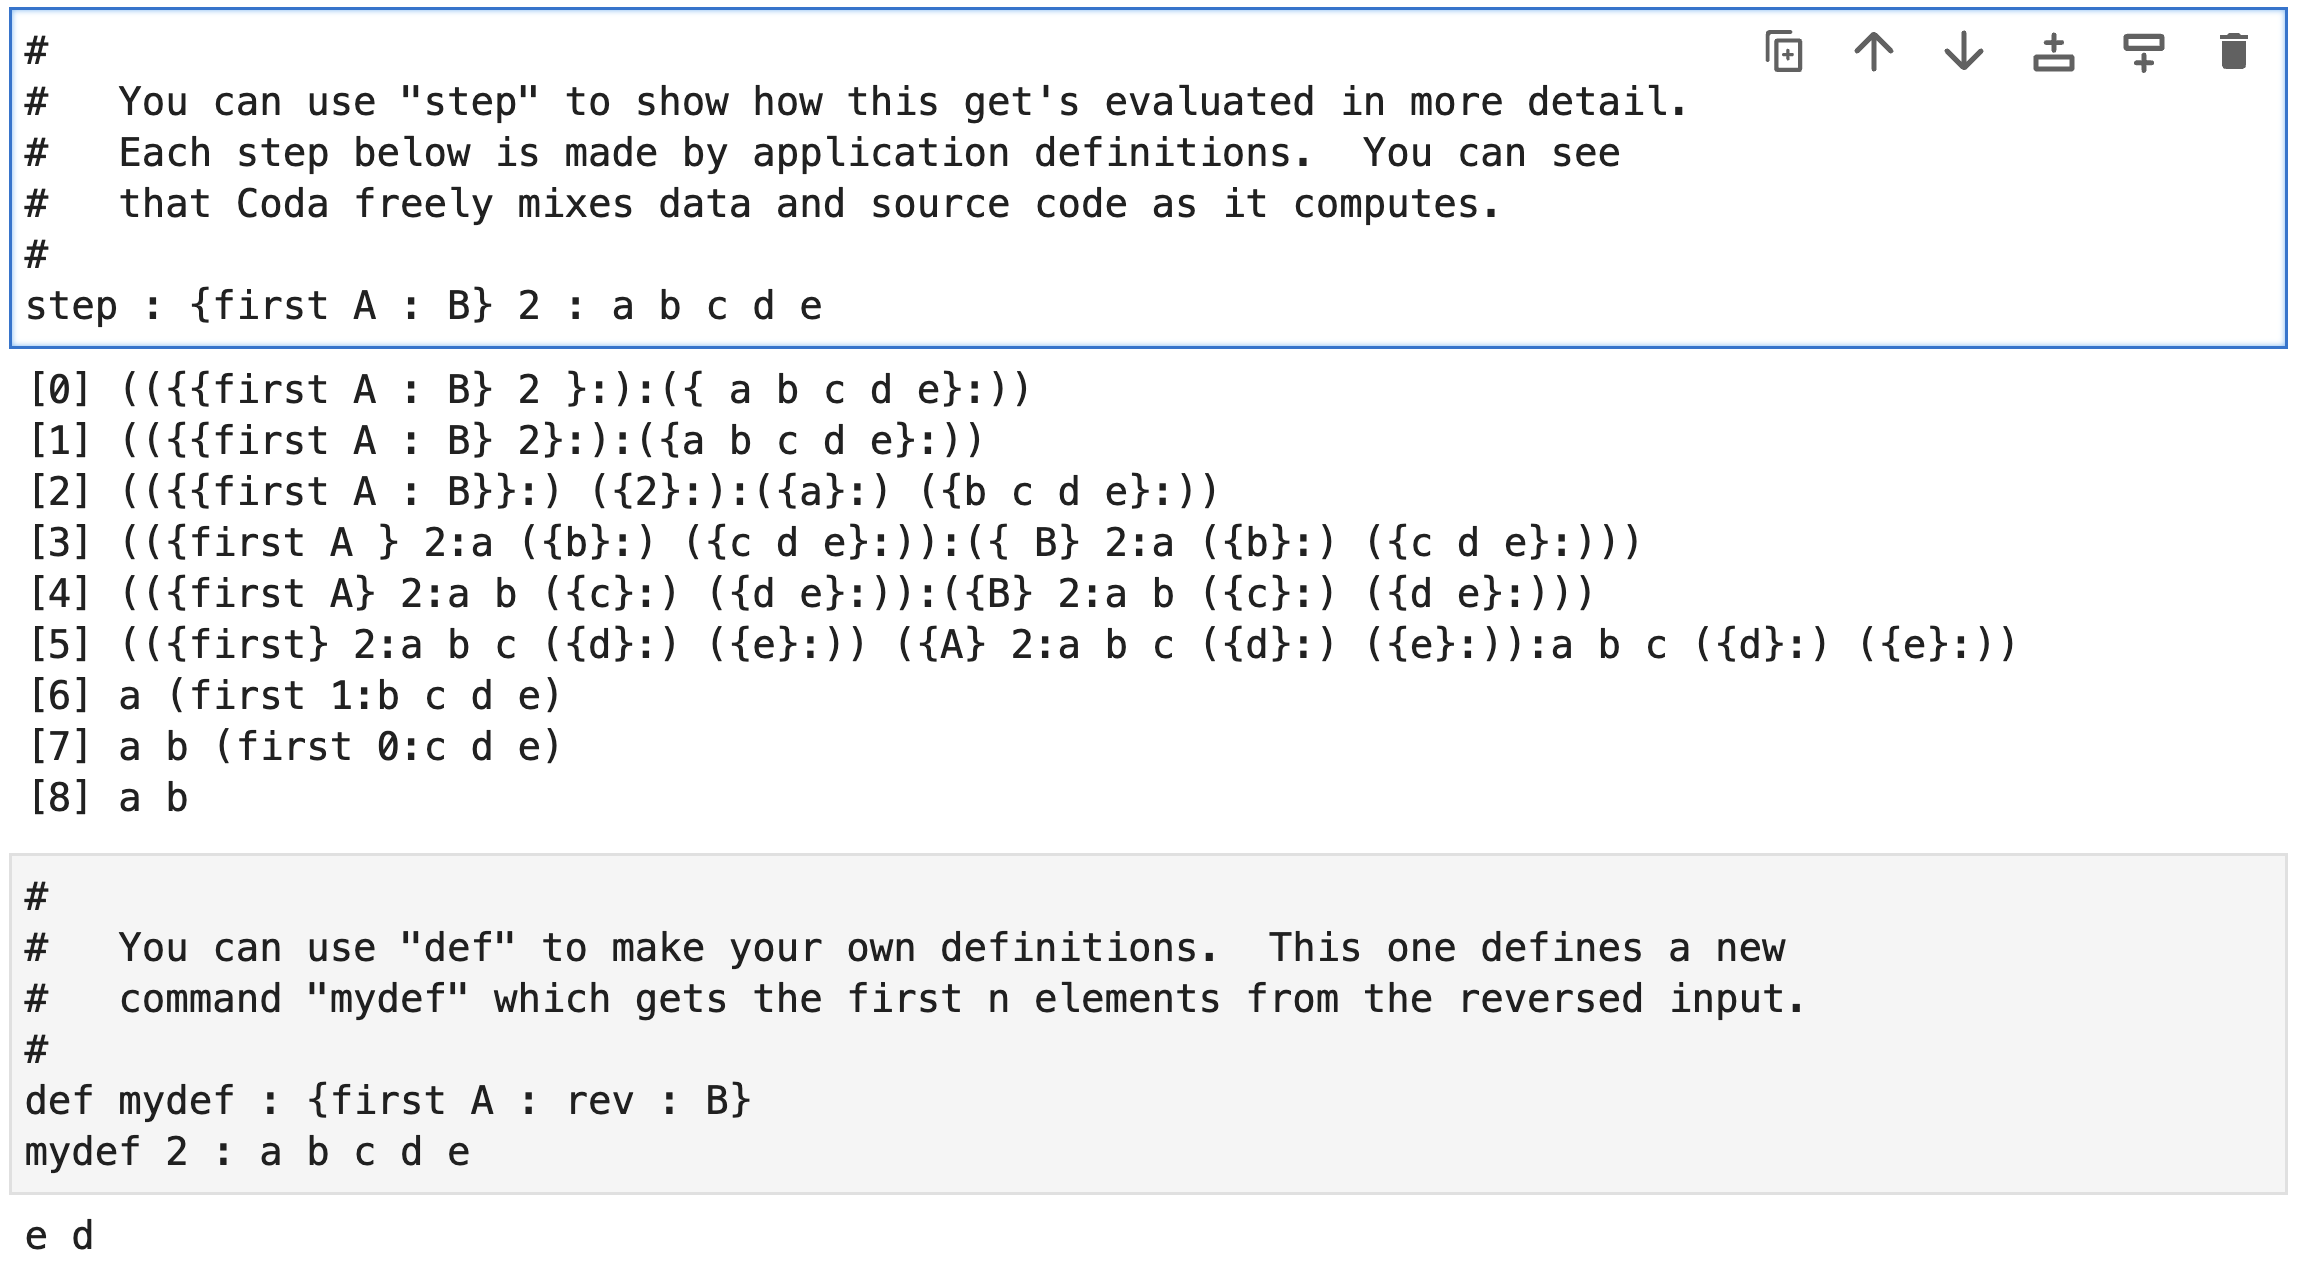
\includegraphics[width=0.9\textwidth]{language_examples.png}
\caption{This is a caption}
\end{figure} 
Figure Y shows an evaluation of the language expression ``step : \{first A : B\} 2 : a b c d e''.  In general, {\it evaluation} means applying 
definitions in some unspecified order.  The {\bf step} definition causes the evaluation to be displayed at each step, showing language expressions 
mixing with other data as the evaluation proceeds.  As shown, the language includes definitions which allow you to create definitions as in the 
example ``def mydef : {first A : rev : B}'' which takes ``input'' (B), reverses the order and then selects the first $n$ items in the reversed sequence 
where $n$ is determined by the ``argument'' A.  

     The language is intentionally a minimalist wrap around the basic algebra of data with a colon and a space for concatenation.   
Only the characters ``{\bf():\{\}=*/\ }" have language significance.  There are no reserved keywords or 
special syntax for variables, functions, classes or exceptions.  The language is unusual in that any byte sequence is a valid language expression.  This means 
that we do not have to specify an alphabet or even define valid and invalid syntax.  There is no such thing 
as invalid syntax.  The source code for the compiler and parser is small enough to be easily read and understood by humans \cite{github}.

\section{Proof and Computation}
\section{Spaces}

\begin{table}
\begin{tabular}{| l | l  | l | l | l | l | }
Space & Action & Data & Space:() & $F*Space=Space*F$ \\
\hline 
pass & A$\rightarrow$A & All data & () & F distributive \\
null & A$\rightarrow$ () & () only & () & F such that F:X=() \\
first & a A$\rightarrow$ a & Single atoms & () & F(a) for atom a \\ 
bool & A$\rightarrow$() $or$ (:) & () or (:) & () & F:X which preserves bool:X \\
type n & A$\rightarrow$ (n:2) (n:1) (n:5) & Natural numbers & () & (type n)$*$F$*$(type n) for any F \\
sum n & (n:2) (n:1) (n:5)$\rightarrow$ (n:8) & Natural numbers & (n:0) & $F(n_1+n_2)=F(n_1)+F(n_2)$ \\
prod n & (n:2) (n:1) (n:5)$\rightarrow$ (n:10) & Natural numbers & (n:1) & $F(n_1*n_2)=F(n_1)*F(n_2)$ \\
sort n & (n:2) (n:1) (n:5)$\rightarrow$ (n:1) (n:2) (n:5) & Natural numbers & () & $n_1\le n_2 \implies F(n_1)\le F(n_2)$ \\
End sum n & $F_1\ F_2\dots F_n\rightarrow F_1*F_2*\dots *F_n$ & Morphisms & pass & Functorial \\
Hom Sum & $F_1\ F_2\dots F_n\rightarrow F_1*F_2*\dots *F_n$ & Morphisms & pass & Functorial \\
\hline
\end{tabular} 
\caption{\label{ }{\it Spaces.}}   
\end{table}


\section{Mathematical Machine Learning}
\section{Is Mathematics Consistent?}
\section{Summary}

%%%%%%%%%%%%%%%%%%%%%%%%%%%%%%%%%%%%%%%%%%%%%%%%%%%%%%%%%%%%%%%%%%%%%%%%
%%% \bibliography{jpsi}
\begin{thebibliography}{10}
\bibitem{github} Source code in github. 
\bibitem{cox} R.T.Cox, Am.J.Phys. 14, 1 (1946).
\bibitem{mpl2} S.Youssef, Mod.Phys.Lett A9, 2571 (1994).
\bibitem{pl} S.Youssef, Phys.Lett. A204, 181(1995).

\end{thebibliography}
%%%%%%%%%%%%%%%%%%%%%%%%%%%%%%%%%%%%%%%%%%%%%%%%%%%%%%%%%%%%%%%%%%%%%%%%
\end{document}
